
\begin{minipage}{.6\textwidth}
	$L = \big\{ \bu.U^+ \otimes U^-\ | \ U = \{u_1 < \cdots < u_{q} \} \in \P_q(n),\ \bu \in \overline{U} \big\}$. \\
	\begin{tab}
		$L^{e} = \{\ind_{\bu.U}(\bu) \text{ even}\}$. 
		\begin{tab}
			$L_{min}^{e} = \{\bu < u_1 \}$.\par
			$\overline{L}_{min}^{e} = L^{e} \setminus L_{min}^{e}$.
			\begin{tab}
				$\overline{L}_{min}^{e,e} =
				\{\ind_{\bu.U}(l_{U}^\bu) \text{ even} \}$. \par
				$\overline{L}_{min}^{e,o} =
				\{\ind_{\bu.U}(l_{U}^\bu) \text{ odd} \}.$ \\
			\end{tab}
		\end{tab}
		$L^{o} = \{\ind_{x.U}(x) \text{ odd}\}$.\par 
		\begin{tab}
			$L_{max}^{o} = \{u_q < \bu\}$.\par
			$\overline{L}_{max}^{o} = L^{o}\setminus L_{max}^{o}$.
			\begin{tab}
				$\overline{L}_{max}^{o,e} = \{\ind_{\bu.U}(r_{U}^\bu) \ \text{even} \}$.\par 
				$\overline{L}_{max}^{o,o} = \{\ind_{\bu.U}(r_{U}^\bu) \ \text{odd}\}$.
			\end{tab}
		\end{tab}
	\end{tab}
\end{minipage}
\begin{minipage}{.4\textwidth}
	\begin{center}
		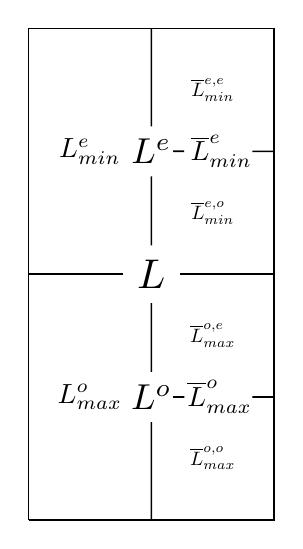
\begin{tikzpicture}[scale = .26]
		\node (L) at (0,0) [scale = 1.5]{$L$};
		\draw [semithick] (-6,0) -- (L) -- (6,0);
		\draw [semithick] (-6,-12) -- (6,-12) -- (6,12) -- (-6,12) -- (-6,-12);
		Statement
		\node (Le) at (0,6) [scale = 1.3] {$L^e$};
		\node (Lemax) at (-3,6) {$ {L}^e_{min}$};
		\node (-Lemax) at (3,6) {$\; \overline{L}^e_{min}$\!\!};
		\node at (3,3) [scale = .7] {$\overline{L}^{e,o}_{min}$};
		\node at (3,9) [scale = .7] {$\overline{L}^{e,e}_{min}$};
		
		\draw [semithick] (L) -- (Le) -- (0,12);
		\draw [semithick] (6,6) -- (-Lemax) -- (Le);
		
		\node (Lo) at (0,-6) [scale = 1.3] {$L^o$};
		\node (Lomin) at (-3,-6) {$ {L}^o_{max}$};
		\node (-Lomin) at (3,-6) {$\, \overline{L}^o_{max}$\!\!};
		\node at (3,-3) [scale = .7] {$\overline{L}^{o,e}_{max}$};
		\node at (3,-9) [scale = .7] {$\overline{L}^{o,o}_{max}$};
		
		\draw [semithick] (L) -- (Lo) -- (0,-12);
		\draw [semithick] (6,-6) -- (-Lomin) -- (Lo);
		\end{tikzpicture}
	\end{center}
\end{minipage}
\ \\

\begin{minipage}{.6\textwidth}
	$R = \big\{ U^+ \otimes \bu.U^- \mid U = \{u_1 < \cdots < u_{q}\} \in \P_q(n), \ \bu \in \overline{U} \big\}$.\\
	\begin{tab}
		$R^{e} = \{\ind_{\bu.U}(\bu) \ \text{even}\}$. \par
		\begin{tab}
			$R_{max}^{e} = \{u_q < \bu\}$. \par 
			$\overline{R}_{max}^{e} = R^{e} \setminus R_{max}^{e}$.
			\begin{tab}
				$\overline{R}_{max}^{e,e} = \{\ind_{\bu.U}(r_{U}^\bu) \ \text{even}\}$. \par 
				$\overline{R}_{max}^{e,o} = \{\ind_{\bu.U}(r_{U}^\bu) \ \text{odd}\}$.\\
			\end{tab}
		\end{tab}
		$R^{o} = \{\ind_{\bu.U}(\bu) \ \text{odd}\}$. \par
		\begin{tab}
			$R_{min}^{o} = \{\bu < u_1\}$. \par
			$\overline{R}_{min}^{o} = R^{o} \setminus R_{min}^{o}$.
			\begin{tab}
				$\overline{R}_{min}^{o,e} = \{\ind_{\bu.U}(l_{U}^\bu) \ \text{even}\}$. \par
				$\overline{R}_{min}^{o,o} = \{\ind_{\bu.U}(l_{U,\bu}) \ \text{odd}\}$.
			\end{tab}
		\end{tab}
	\end{tab}
\end{minipage}
\begin{minipage}{.4\textwidth}
	\begin{center}
		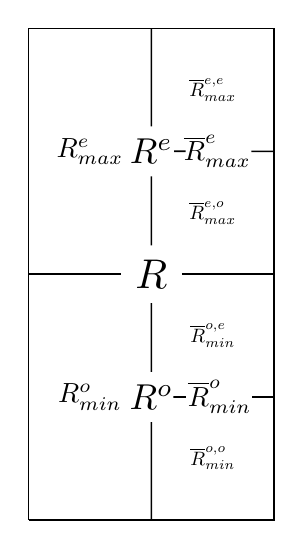
\begin{tikzpicture}[scale = .26]
		\node (L) at (0,0) [scale = 1.5]{$R$};
		\draw [semithick] (-6,0) -- (L) -- (6,0);
		\draw [semithick] (-6,-12) -- (6,-12) -- (6,12) -- (-6,12) -- (-6,-12);
		
		\node (Le) at (0,6) [scale = 1.3] {$R^e$};
		\node (Lemax) at (-3,6) {$ {R}^e_{max}$};
		\node (-Lemax) at (3,6) {$\overline{R}^e_{max}$\!\!};
		\node at (3,3) [scale = .7] {$\overline{R}^{e,o}_{max}$};
		\node at (3,9) [scale = .7] {$\overline{R}^{e,e}_{max}$};
		
		\draw [semithick] (L) -- (Le) -- (0,12);
		\draw [semithick] (6,6) -- (-Lemax) -- (Le);
		
		\node (Lo) at (0,-6) [scale = 1.3] {$R^o$};
		\node (Lomin) at (-3,-6) {$ {R}^o_{min}$};
		\node (-Lomin) at (3,-6) {\,$\overline{R}^o_{min}$\!\!};
		\node at (3,-3) [scale = .7] {$\overline{R}^{o,e}_{min}$};
		\node at (3,-9) [scale = .7] {$\overline{R}^{o,o}_{min}$};
		
		\draw [semithick] (L) -- (Lo) -- (0,-12);
		\draw [semithick] (6,-6) -- (-Lomin) -- (Lo);
		\end{tikzpicture}
	\end{center}
\end{minipage}\\
